\documentclass[journal,twoside]{IEEEtran}
\usepackage{amsmath}
\usepackage{amssymb}
\interdisplaylinepenalty=2500
\usepackage[dvips]{graphicx}
\newtheorem{definition}{Definition}

\begin{document}
\bibliographystyle{IEEEtran.bst}

\title{Mixed Data-Type Circuit Modeling:\\ The Ideal Diode}
\author{XXXXX
\thanks{The author is with the XXXXX.}}
\markboth{Article Preprint: August 2004}{XXXXX: A Mixed Data-Type Algebra for Circuit Modeling}
\maketitle

\begin{abstract}
This article presents a mixed numeric plus Boolean data-type algebraic representation that can be used to characterize certain non-linear ideal circuit components for the purpose of sparse matrix circuit modeling.
The first part of this article introduces the concept of and some features of a mixed data-type algebra in the context of electronics.  
Then a mixed data-type characterization for the ideal diode is presented. 
Finally the mixed data-type models of several example circuits are explored. 
\end{abstract}

\section{Introduction}
\PARstart{T}he use of mixed data-type expressions, although not commonly used in mathematics of electronics engineering,  is included in the syntax of the C and C++ computer programming languages \cite{bk:c,sd:cpp,bs:cpp}.
We will build on that source as well as on the notational conventions and syntax used in discrete and foundational mathematics \cite{sg:dfm} to develop a mixed data-type algebra for circuit modeling.

In most engineering contexts it is implicitly understood that the data-type of a constant or unknown variable is a real number.
The algebraic expressions that use these variables include operators that are defined for real numbers, such as ``+" for addition and the blank no symbol at all for multiplication.
The resultant data-type of an algebraic expression such as $a+b$ is then subsequently understood to be a real number.
This is symbolically indicated by $(a+b) \in \mathbb R$. 
When it is said that division by zero is not defined it means that whatever the result of division by zero is, it is not a real number.
 
Additionally, the specialized engineering context of logic circuit design employs the Boolean ``true" or ``false" data-type\footnote[1]{The Boolean data-type is alternatively sometimes thought of as a binary numeric data-type.}.
The Boolean data-type as used in engineering has its own collection of operators including ``+" for logical OR and ``$\times $" (or again no symbol at all) for logical AND.
In this context the resultant data-type of an algebraic expression such as $a+b$ is understood to be Boolean.
This is symbolically indicated by $(a+b) \in \mathbb B$.
The reuse and redefinition of operator symbols for different data-types is known as \emph{operator overloading}.

\section{Mixed data-type expressions} It is possible to construct mixed data-type expressions if we define rules for automatic \emph{type conversion}.
To avoid ambiguity we will for the most part not overload operators in this presentation. 
We will use the logical operator symbol set from pure mathematics which includes, for example, ``$\wedge$" for logical AND and ``$\vee$" for logical OR.

We define a type conversion scheme in which the Boolean data-type is converted to a numeric data type.
The type conversion is automatically invoked whenever an operator requires a real number but has been given a Boolean value.
The type conversion rule is quite simple: 
\begin{quote}
\emph{When required, convert the Boolean ``true" to the real number 1 and the Boolean ``false" to the real number 0.}
\end{quote}
This is the only type conversion that will be required in the application presented in this article.

Given a real number type variable $a$ and a Boolean variable $b$, again consider the algebraic expression $a+b$.
Since the + operator is now only defined for real numbers it is necessary to convert the Boolean type variable $b$ to a numeric value for expression to be defined. 
If, for example, the value of $a$ is 5 and the value of $b$ is true, the value of the expression $a+b$ is 6.
The expression has a resultant real number data-type.

The operators ``+" for addition and ``$\wedge$" for logical AND are \emph{binary operators} in the sense that they take two inputs.
The addition operator takes two numeric input values and produces one numeric output value.
The logical AND operator takes two Boolean input values and produces one Boolean output value.
Somewhat differently, the greater-than operator ``$>$" takes two numeric input values and produces one Boolean output value.
So, using our type conversion rule, the resultant data-type of the expression $c\,(a>b)$ is numeric.
If, for example, the value of $a$ is 2, the value of $b$ is 1 and the value of $c$ is 5, the value of the expression $c\,(a>b)$ is 5.

\begin{table}
\begin{center}
\begin{tabular}{|c|l|l|l|l|}
\hline Operator & Operation & \multicolumn{2}{l|}{Arguments} & Result \\
\hline + & addition & numeric & numeric & numeric\\
\hline - & subtraction & numeric & numeric & numeric\\
\hline - & negation & numeric & none & numeric\\
\hline (blank) & multiplication &  numeric & numeric & numeric\\
\hline  / & division &  numeric & numeric & numeric\\
\hline  $<$ & less than &  numeric & numeric & boolean\\
\hline  $>$ & greater than &  numeric & numeric & boolean\\
\hline  $=$ & equal to &  numeric & numeric & boolean\\
\hline  $\wedge$ & and &  boolean & boolean & boolean\\
\hline  $\vee$ & or &  boolean & boolean & boolean\\
\hline  $\oplus $ & exclusive or &  boolean & boolean & boolean\\
\hline $\Rightarrow$ & implication & boolean & boolean & boolean\\
\hline
\end{tabular}
\end{center}
\caption{Operators}
\end{table}

Table \arabic{table} gives a summary of all the operators that we will use.
Note that we have overloaded the ``$-$" operator, using it as the symbol for both the binary operation subtraction and for the unary operation negation.

Using our notational convention as defined so far, the expression $i=v/R$, where $(i,v,R) \in \mathbb R$,  evaluates to a Boolean data-type, and as such could be either true or false.
If we are intending to make a statement of Ohm's Law, what we would actually want to say is that for all possible values of $i$, $v$ and $R$ this expression is always true. 
A statement consisting of an \emph{always true} boolean expression is known as a \emph{tautology}. 
The symbol $\vDash$ is used to indicate that the statement it precedes is a tautology.
Ohm's Law expressed as tautological statement is:   
\begin{equation*}
\vDash (i=v/R)
\end{equation*}
For the sake of brevity we will often omit the symbol $\vDash$ and refer to a tautological statement simply as a \emph{statement} to distinguish it from an \emph{expression}.

%We will place the symbol $\equiv$ between two expressions to indicate that the expressions are \emph{equivalent} to each other.
%For example, a new boolean variable $r$ is introduced by the statement:
%\begin{equation*}
%r \equiv (i>0)
%\end{equation*}
%Any expression can be replaced by it's equivalent and, as we will see, the simplification resulting from substitution of an equivalent can be usefull.

Expressions in the following form will reoccur later in this article: 
\begin{gather*}
rx + sy = c\\
\text{where }  (r,s) \in \mathbb B , \: (x,y,c) \in \mathbb R \\
\text{and } \vDash (r \oplus s)
\end{gather*}
In this case we will refer to the boolean variables $r$ and $s$ as \emph{selectors} since they effectively select one of the numeric variables $x$ or $y$ as being equal to the constant number $c$. 

\section{Characteristic statements}
Electronic devices as mathematical entities are defined by their characteristic tautological statements \cite{ru:css}. 
From this perspective Ohm's Law is simply the characterization statement for the resistor device. 
Device characteristic statements are the building blocks that we use to create circuit models.
A circuit model is also, in turn, as a whole, a larger compound tautological statement. 

When doing circuit modeling with a sparse matrix \cite{ru:css}, as we will in this article, it is easier to work with the matrix formulation of device characteristic statements.
For the resistor device as an example we have:
\begin{gather*}
\begin{bmatrix} 1 & -R \end{bmatrix}
\begin{bmatrix} v \\ i \end{bmatrix}=0
\end{gather*}
 
Next we will use mixed data-type statements to characterize the ideal diode.
 
\section{The ideal diode}
\begin{figure}[ht]
\centering
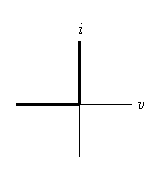
\includegraphics{d1full}
\caption{Diode characteristic $vi$ curve.}
\label{fig:diode}
\end{figure}

Figure \ref{fig:diode} is a plot of the characteristic $vi$ curve for an ideal diode.
This curve is clearly non-linear.
Additionally, because the curve is 'L' shaped and aligned with both axis, it cannot be represented as a piece-wise linear function.  
However, it is possible to build a mixed data-type representation based on the observations that:
\begin{enumerate}
\item either the voltage or the current is zero,
\item if the current is zero then the voltage is less than or equal to zero,
\item and if the voltage is zero then the current is greater than or equal to zero.
\end{enumerate}
These observations can be represented symbolically with the mixed data-type expressions:
\begin{gather*}
(v=0) \vee (i=0) \\
(i=0) \Rightarrow (v \le 0) \\
(v=0) \Rightarrow (i \ge 0)
\end{gather*}
These three expressions can be combined to give a single complete mixed data-type characteristic statement for the ideal diode:
\begin{multline*}\vDash \Big(
\big((v=0) \vee (i=0)\big) \wedge \\
\big((i=0) \Rightarrow (v \le 0)\big) \wedge \\
\big((v=0) \Rightarrow (i \ge 0)\big) \Big)
\end{multline*}

The ideal diode can also be equivalently characterized using selector notation and the following collection of statements:
\begin{gather}
rv + si=0 \label{eq:d1}\\
r \oplus s \label{eq:d2}\\
(i=0) \Rightarrow (v \le 0) \label{eq:d3}\\
(v=0) \Rightarrow (i \ge 0) \label{eq:d4}
\end{gather}
In matrix form equations (\ref{eq:d1}) and (\ref{eq:d2}) become:
\begin{gather}
\begin{bmatrix} r & s \end{bmatrix}
\begin{bmatrix} v \\ i \end{bmatrix}=0 \label{eq:dsel1} \\
\text{where }\begin{bmatrix} r & s \end{bmatrix} 
\in \left\{ \begin{bmatrix} 0 & 1 \end{bmatrix},
\begin{bmatrix} 1 & 0 \end{bmatrix} \right\} \label{eq:dsel2}
\end{gather}
Note that when the diode current is non-zero we say that the diode is \emph{forward biased} and when the voltage is non-zero we say that the diode is \emph{reverse biased}.

\section{Circuit modeling with the ideal diode}
The next goal will be to use the mixed data-type characterization of the ideal diode as  a building block in a circuit model.

\begin{figure}[ht]
\centering
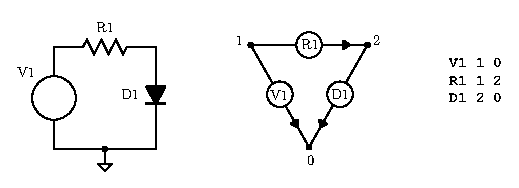
\includegraphics{c1}
\caption{Example circuit.}
\label{fig:ex1}
\end{figure}
\subsection{Single diode example.}Figure \ref{fig:ex1} shows schematic, a digraph, and a netlist for an example circuit.
An electrical engineer could readily produce mathematical statements for the diode voltage drop and diode current by inspection for this simple circuit.
What we seek however is a general method for finding solutions that proceeds mechanically in a way that is conducive to computer implementation.

Using the method and conventions given in \cite{ru:css}, the symbolic sparse matrix model in the form $[ \mathbf T| \mathbf u]$ for this example is:
\begin{gather}
\left[\begin{array}{cccccccc|c}
0 &0 &0 &0 &0 &1 &1 &0 &0\\
0 &0 &0 &0 &0 &0 &-1 &1 &0\\
-1 &0 &1 &0 &0 &0 &0 &0 &0\\
-1 &1 &0 &1 &0 &0 &0 &0 &0\\
0 &-1 &0 &0 &1 &0 &0 &0 &0\\
0 &0 &1 &0 &0 &0 &0 &0 &V_{V1}\\
0 &0 &0 &1 &0 &0 &-R_{R1} &0 &0\\
0 &0 &0 &0 &r_{D1} &0 &0 &s_{D1} &0
\end{array}\right]
\label{eq:ag1}
\end{gather}\\
Note that selectors for the diode have been included in the model thereby creating a mixed data-type augmented matrix.
As a first check for the existence of solutions, we calculate\footnote[1]{The author has used the software package \emph{Maple} \cite{wm:maple} to assist with many of the symbolic calculations in this article.} the determinant of the left-hand side of the augmented matrix and get the result:
\begin{gather*}
\det \mathbf T = s_{D1}-r_{D1}R_{R1}
\end{gather*}
Solutions to the model exist only when the determinant is non-zero.
Remembering the selector cases given in equation (\ref{eq:dsel2}), we begin the construction of a solutions table by listing all of the possible selector values along with the associated determinant value:
\begin{gather*}
\begin{array}{l|c}
\left[ \; r_{D1} \; \; s_{D1} \; \right] &\det \mathbf T \\ \hline
\left[ \; 0 \; \; 1 \; \right] &1 \\
\left[ \; 1 \; \; 0 \; \right] &-R_{R1}
%[ \; 1 \; \; 0 \; ] &-R_{R1}
\end{array}
\end{gather*}\\
To insure that the determinant is non-zero, we need to append a constraint to the second row in the solutions table:
\begin{gather*}
\begin{array}{l|c|l}
\left[ \; r_{D1} \; \; s_{D1} \; \right] &\det \mathbf T &\text{constraints} \\ \hline
\left[ \; 0 \; \; 1 \; \right] &1 &\text{none} \\
\left[ \; 1 \; \; 0 \; \right] &-R_{R1} &R_{R1} > 0 
\end{array}
\end{gather*}\\
Note that we have also taken into account the global constraint that all resistors are non-negative.

Solving the model matrix (\ref{eq:ag1}) symbolically for the diode voltage drop and diode current  solution variables yields:
\begin{gather*}
v_{D1}=\frac{s_{D1}V_{V1}}{\det \mathbf T} \\ \\
i_{D1}=\frac{-r_{D1}V_{V1}}{\det \mathbf T} \\
\end{gather*}
We refine the solutions table by adding a column for each of the desired solution variables and removing the now redundant determinant column: 
\begin{gather*}
\begin{array}{l|c|c|c}
\left[ \; r_{D1} \; \; s_{D1} \; \right] &\text{constraints} &v_{D1} &i_{D1} \\ \hline
\left[ \; 0 \; \; 1 \; \right] &\text{none} &V_{V1} &0 \\
\left[ \; 1 \; \; 0 \; \right] &R_{R1} > 0 &0 &V_{V1}/R_{R1} 
\end{array}
\end{gather*}\\
Note that at this stage we could have added a column for any other desired solution variable such as, for example, resistor current. 
Next we remove the redundant selectors column and include any additional constraints based on the implication of the diode characterization statements (\ref{eq:d3}) and (\ref{eq:d4}):
\begin{gather*}
\begin{array}{c|c|c}
\text{constraints} &v_{D1} &i_{D1} \\ \hline
v_{D1} \le 0 &V_{V1} &0 \\
i_{D1} \ge 0, R_{R1} > 0 &0 &V_{V1}/R_{R1} 
\end{array}
\end{gather*}\\
Finally we seek to express everything in the constraints column in a form that does not contain any of the solution variables.
In the first solution row we have the constraint $v_{D1} \le 0$. But since the second column gives $v_{D1} = V_{V1}$ this constraint can be equivalently expressed as $V_{V1} \le 0$.
In a similar manner we also replace the first constraint in the second row.
The complete solutions table for the sample circuit is:
\begin{gather*}
\begin{array}{c|c|c}
\text{constraints} &v_{D1} &i_{D1} \\ \hline
V_{V1} \le 0 &V_{V1} &0 \\
V_{V1} \ge 0, R_{R1} > 0 &0 &V_{V1}/R_{R1} 
\end{array}
\end{gather*}\\
Note that there is a case under which the model does not give a solution, namely when $V_{V1} > 0$ and $R_{R1} = 0$.
In this case the problem is that a zero value resistor would result in an infinite current.

All of the diode voltage drop and diode current solutions for this example circuit are therefore given by the equivalent single complete mixed data-type statement:
\begin{multline*}\vDash \Big(
\big((V_{V1} \!\le \! 0)  \!\implies \! (v_{D1} \!= \!V_{V1})  \!\wedge \! (i_{D1} \!= \!0)\big)  \!\wedge \! \\
\big((V_{V1}  \!>\! 0)  \!\wedge \! (R_{R1} > 0)  \!\implies \! (v_{D1} \!= \!0)  \!\wedge \! (i_{D1} \!= \!V_{V1}/R_{R1})\big)
\Big)\end{multline*}
Notice that in this statement we have removed the overlap in cases where $V_{V1}  = 0$.

\begin{figure}[ht]
\centering
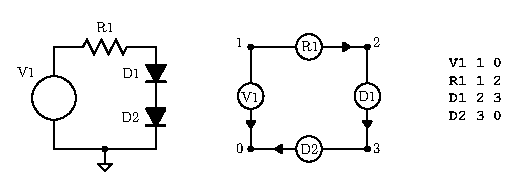
\includegraphics{c2}
\caption{Example circuit.}
\label{fig:ex2}
\end{figure}

\subsection{A series diode example.}Figure \ref{fig:ex2} shows schematic, a digraph, and a netlist for a series diode example circuit.
Proceeding as before, the determinant for the model is given by:
\begin{gather*}
\det \mathbf T = -s_{D2}r_{D1}-s_{D1}r_{D2}+r_{D1}r_{D2}R_{R1}
\end{gather*}
Construction of the solutions table begins as a list of all of the possible selector cases along with the associated determinant value:
\begin{gather*}
\begin{array}{c|c}
\left[ \; r_{D1} \; \; s_{D1} \;\; r_{D2} \; \; s_{D2} \; \right] &\det \mathbf T \\ \hline
\left[ \; 0 \;\; 1 \;\; 0 \;\; 1 \; \right] &0 \\
\left[ \; 0 \;\; 1 \;\; 1 \;\; 0 \; \right] &-1 \\
\left[ \; 1 \;\; 0 \;\; 0 \;\; 1 \; \right] &-1 \\
\left[ \; 1 \;\; 0 \;\; 1 \;\; 0 \; \right] &R_{R1}
\end{array}
\end{gather*}\\
Solutions occur only when the determinant is non-zero, so we delete the first row and append constraints as required:
\begin{gather*}
\begin{array}{c|c|l}
\left[ \; r_{D1} \; \; s_{D1} \;\; r_{D2} \; \; s_{D2} \; \right] &\det \mathbf T &\text{constraints} \\ \hline
\left[ \; 0 \;\; 1 \;\; 1 \;\; 0 \; \right] &-1 &\text{none} \\
\left[ \; 1 \;\; 0 \;\; 0 \;\; 1 \; \right] &-1 &\text{none} \\
\left[ \; 1 \;\; 0 \;\; 1 \;\; 0 \; \right] &R_{R1} &R_{R1} > 0 
\end{array}
\end{gather*}\\
Solving the model matrix symbolically for the diode voltage drop and diode current  solution variables yields:
\begin{gather*}
v_{D1}=\frac{-s_{D1}r_{D2}V_{V1}}{\det \mathbf T} \\ \\
i_{D1}=\frac{r_{D1}r_{D2}V_{V1}}{\det \mathbf T} \\ \\
v_{D2}=\frac{-r_{D1}s_{D2}V_{V1}}{\det \mathbf T} \\ \\
i_{D2}=\frac{r_{D1}r_{D2}V_{V1}}{\det \mathbf T} \\
\end{gather*}
We refine the solutions table by removing both the selectors column and the determinant column and adding a column for each of the desired solution variables: 
\begin{gather*}
\begin{array}{c|c|c|c|c}
\text{constraints} &v_{D1} &i_{D1} &v_{D2} &i_{D2} \\ \hline
\text{none} &V_{V1} &0 &0 &0 \\
\text{none} &0 &0 &V_{V1} &0 \\
R_{R1} > 0 &0 &V_{V1}/R_{R1} &0 &V_{V1}/R_{R1} 
\end{array}
\end{gather*}\\
Next we update the constraints based on the diode characterization implications:
\begin{gather*}
\begin{array}{c|c|c|c|c}
\text{constraints} &v_{D1} &i_{D1} &v_{D2} &i_{D2} \\ \hline
v_{D1} \le 0 &V_{V1} &0 &0 &0 \\ \hline
v_{D2} \le 0 &0 &0 &V_{V1} &0 \\ \hline
\begin{array}{ccc}
i_{D1} \ge 0, \\
i_{D2} \ge 0, \\
R_{R1} > 0
\end{array} &0 &V_{V1}/R_{R1} &0 &V_{V1}/R_{R1} 
\end{array}
\end{gather*}\\
After expressing everything in the constraints column in a form that does not contain any of the solution variables we have:
\begin{gather*}
\begin{array}{c|c|c|c|c}
\text{constraints} &v_{D1} &i_{D1} &v_{D2} &i_{D2} \\ \hline
V_{V1} \le 0 &V_{V1} &0 &0 &0 \\ \hline
V_{V1} \le 0 &0 &0 &V_{V1} &0 \\ \hline
\begin{array}{ccc}
V_{V1} \ge 0, \\
R_{R1} > 0
\end{array} &0 &V_{V1}/R_{R1} &0 &V_{V1}/R_{R1} 
\end{array}
\end{gather*}\\
The first two rows contradict each other except when $V_{V1}=0$.
We can remove the contradiction by tightening the constraints and combining the first two rows.
The completed solutions table is:
\begin{gather*}
\begin{array}{c|c|c|c|c}
\text{constraints} &v_{D1} &i_{D1} &v_{D2} &i_{D2} \\ \hline
V_{V1} = 0 &0 &0 &0 &0 \\ \hline
\begin{array}{ccc}
V_{V1} \ge 0, \\
R_{R1} > 0
\end{array} &0 &V_{V1}/R_{R1} &0 &V_{V1}/R_{R1} 
\end{array}
\end{gather*}

There are cases under which the model does not give a solution.
When $V_{V1} < 0$ the voltage at the node common to the diodes is apparently not well-defined.
This problem could be resolved in practice by simply not using series ideal diodes in the model.
Replacing series diodes with a single ideal diode gives a more comprehensive and overall no less informative solution.
When $V_{V1} > 0$ and $R_{R1} = 0$ there is still a problem however with the resultant infinite current.

All of the diode voltage drop and diode current solutions for this example circuit are given by the single complete mixed data-type statement:
\begin{multline*}\vDash \Big(
\big((V_{V1} \!=\! 0)  \!\implies \! (v_{D1} \!=\! i_{D1} \!=\! v_{D2} \!=\! i_{D2} \!=\! 0)\big)  \!\wedge \! \\
\big((V_{V1} \!>\! 0)  \!\wedge\! (R_{R1} > 0)  \!\implies \! \\
(v_{D1} \!=\! v_{D2} \!=\! 0)  \!\wedge\! (i_{D1} \!=\! i_{D2} \!=\! V_{V1}/R_{R1})\big)
\Big)\end{multline*}
Notice that we have removed the overlap in cases where $V_{V1}  = 0$.

\begin{figure}[ht]
\centering
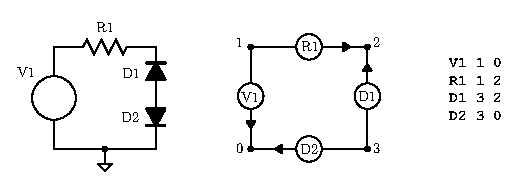
\includegraphics{c3}
\caption{Example circuit.}
\label{fig:ex3}
\end{figure}

\subsection{A back-to-back diode example.}Figure \ref{fig:ex3} shows schematic, a digraph, and a netlist for a back-to-back diode example circuit.
The determinant and the beginning solutions table for the model are the same as in the previous example:
\begin{gather*}
\det \mathbf T = -s_{D2}r_{D1}-s_{D1}r_{D2}+r_{D1}r_{D2}R_{R1}
\end{gather*}
\begin{gather*}
\begin{array}{c|c}
\left[ \; r_{D1} \; \; s_{D1} \;\; r_{D2} \; \; s_{D2} \; \right] &\det \mathbf T \\ \hline
\left[ \; 0 \;\; 1 \;\; 0 \;\; 1 \; \right] &0 \\
\left[ \; 0 \;\; 1 \;\; 1 \;\; 0 \; \right] &-1 \\
\left[ \; 1 \;\; 0 \;\; 0 \;\; 1 \; \right] &-1 \\
\left[ \; 1 \;\; 0 \;\; 1 \;\; 0 \; \right] &R_{R1}
\end{array}
\end{gather*}\\
As in the previous example we delete the first row and append constraints as required:
\begin{gather*}
\begin{array}{c|c|l}
\left[ \; r_{D1} \; \; s_{D1} \;\; r_{D2} \; \; s_{D2} \; \right] &\det \mathbf T &\text{constraints} \\ \hline
\left[ \; 0 \;\; 1 \;\; 1 \;\; 0 \; \right] &-1 &\text{none} \\
\left[ \; 1 \;\; 0 \;\; 0 \;\; 1 \; \right] &-1 &\text{none} \\
\left[ \; 1 \;\; 0 \;\; 1 \;\; 0 \; \right] &R_{R1} &R_{R1} > 0 
\end{array}
\end{gather*}\\
Solving the model matrix symbolically for the diode voltage drop and diode current  solution variables yields:
\begin{gather*}
v_{D1}=\frac{s_{D1}r_{D2}V_{V1}}{\det \mathbf T} \\ \\
i_{D1}=\frac{-r_{D1}r_{D2}V_{V1}}{\det \mathbf T} \\ \\
v_{D2}=\frac{-r_{D1}s_{D2}V_{V1}}{\det \mathbf T} \\ \\
i_{D2}=\frac{r_{D1}r_{D2}V_{V1}}{\det \mathbf T} \\
\end{gather*}
We refine the solutions table by removing both the selectors column and the determinant column and adding a column for each of the desired solution variables: 
\begin{gather*}
\begin{array}{c|c|c|c|c}
\text{constraints} &v_{D1} &i_{D1} &v_{D2} &i_{D2} \\ \hline
\text{none} &-V_{V1} &0 &0 &0 \\
\text{none} &0 &0 &V_{V1} &0 \\
R_{R1} > 0 &0 &V_{V1}/R_{R1} &0 &-V_{V1}/R_{R1} 
\end{array}
\end{gather*}\\
Next we update the constraints based on the diode characterization implications:
\begin{gather*}
\begin{array}{c|c|c|c|c}
\text{constraints} &v_{D1} &i_{D1} &v_{D2} &i_{D2} \\ \hline
v_{D1} \le 0 &-V_{V1} &0 &0 &0 \\ \hline
v_{D2} \le 0 &0 &0 &V_{V1} &0 \\ \hline
\begin{array}{ccc}
i_{D1} \ge 0, \\
i_{D2} \ge 0, \\
R_{R1} > 0
\end{array} &0 &V_{V1}/R_{R1} &0 &-V_{V1}/R_{R1} 
\end{array}
\end{gather*}\\
After expressing everything in the constraints column in a form that does not contain any of the solution variables we have:
\begin{gather*}
\begin{array}{c|c|c|c|c}
\text{constraints} &v_{D1} &i_{D1} &v_{D2} &i_{D2} \\ \hline
V_{V1} \ge 0 &-V_{V1} &0 &0 &0 \\ \hline
V_{V1} \le 0 &0 &0 &V_{V1} &0 \\ \hline
\begin{array}{ccc}
V_{V1} \ge 0, \\
V_{V1} \le 0, \\
R_{R1} > 0
\end{array} &0 &V_{V1}/R_{R1} &0 &-V_{V1}/R_{R1} 
\end{array}
\end{gather*}\\
Combining constraints in the third row gives:
\begin{gather*}
\begin{array}{c|c|c|c|c}
\text{constraints} &v_{D1} &i_{D1} &v_{D2} &i_{D2} \\ \hline
V_{V1} \ge 0 &-V_{V1} &0 &0 &0 \\ \hline
V_{V1} \le 0 &0 &0 &V_{V1} &0 \\ \hline
\begin{array}{ccc}
V_{V1} = 0, \\
R_{R1} > 0
\end{array} &0 &0 &0 &0 
\end{array}
\end{gather*}\\
But since the case represented by the third row is also given in both the first and second row, we can delete the third row. 
The final solutions table is:
\begin{gather*}
\begin{array}{c|c|c|c|c}
\text{constraints} &v_{D1} &i_{D1} &v_{D2} &i_{D2} \\ \hline
V_{V1} \ge 0 &-V_{V1} &0 &0 &0 \\ \hline
V_{V1} \le 0 &0 &0 &V_{V1} &0
\end{array}
\end{gather*}\\
The model gives solutions for all cases.
Note that there are no conditions under which current flows in this circuit.

All of the diode voltage drop and diode current solutions for this example circuit are given by the single complete mixed data-type statement:
\begin{multline*}\vDash \Big(
\big((V_{V1} \!=\! 0)  \!\implies \! (v_{D1} \!=\! i_{D1} \!=\! v_{D2} \!=\! i_{D2} \!=\! 0)\big)  \!\wedge \! \\
\big((V_{V1} \!>\! 0)  \!\implies \! 
(v_{D1} \!=\! -V_{V1})  \!\wedge\! (i_{D1} \!=\! i_{D2} \!=\! v_{D2} \!=\! 0)
\wedge \! \\
\big((V_{V1} \!<\! 0)  \!\implies \! 
(v_{D2} \!=\! V_{V1})  \!\wedge\! (i_{D1} \!=\! i_{D2} \!=\! v_{D1} \!=\! 0)\big)
\Big)\end{multline*}

\begin{figure}[ht]
\centering
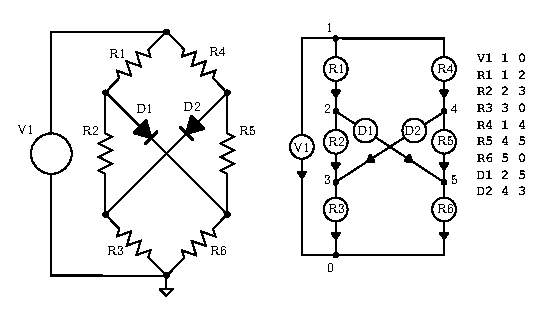
\includegraphics{c4}
\caption{Example circuit.}
\label{fig:ex4}
\end{figure}

\subsection{A more complex example with two diodes.}Figure \ref{fig:ex4} shows schematic, a digraph, and a netlist for another example circuit. 
It is relatively easy to identify by inspection the conditions under which both diodes would be forward biased (ie: current is non-zero).
But let's ask a somewhat more difficult question:\\[10pt]
\emph{Under what conditions, if any, will diode $D1$ be forward biased and diode $D2$ be reverse biased?}\\ 

To answer this question we will concentrate only on the one required row in the solutions table.
The row associated with the case where diode $D1$ current is non-zero and diode $D2$ voltage is non-zero is the row in which:
\begin{gather*}
\left[ \; r_{D1} \; \; s_{D1} \;\; r_{D2} \; \; s_{D2} \; \right] =
\left[ \; 1 \;\; 0 \;\; 0 \;\; 1 \; \right]
\end{gather*}
The determinant evaluated for this row is given by:
\begin{multline*}
\det \mathbf T = R_{R1}(R_{R2} + R_{R3})(R_{R4} + R_{R5}+ R_{R6}) + \\
R_{R6}(R_{R4} + R_{R5})(R_{R1} + R_{R2}+ R_{R3})
\end{multline*}
Note that because resistors have non-negative values, the determinant is also non-negative. 
There are a number of combinations of zero valued resistors that will cause the determinant to be zero.
This row will therefore not give a solution under any of the following conditions:
\begin{gather}
R_{R1} + R_{R2}+ R_{R3} = 0 \label{eq:cf}\\
R_{R4} + R_{R5}+ R_{R6} = 0 \\
R_{R1} + R_{R4}+ R_{R5} = 0 \\
R_{R2} + R_{R3}+ R_{R6} = 0 \\
R_{R1} + R_{R6} = 0 \\
R_{R2} + R_{R3}+ R_{R4} + R_{R5}= 0 \label{eq:cl}
\end{gather}

We continue by considering the voltage and current associated with diode $D2$ as evaluated for the row under consideration:
\begin{multline*}
v_{D2} =
V_{V1}
(R_{R1}R_{R2}R_{R5}+
R_{R1}R_{R2}R_{R6}+
R_{R1}R_{R3}R_{R5}+\\
R_{R1}R_{R5}R_{R6}+
R_{R2}R_{R4}R_{R6}+
R_{R2}R_{R5}R_{R6}) / \det \mathbf T
\end{multline*}
But since the current $i_{D2}$ is evaluated to be zero, the diode characteristic implication (\ref{eq:d3}) states that voltage $v_{D2}$ must be less than or equal to zero.
Because the determinant is positive and resistors have non-negative values, this in turn implies that
\begin{gather} 
V_{V1} \le 0 
\label{eq:db1}
\end{gather}
and this becomes a new constraint for the row. 

Now we consider the current and voltage associated with diode $D1$ as evaluated for this row:
\begin{multline*}
i_{D1} =
V_{V1}
(R_{R2}R_{R4}+
R_{R2}R_{R5} + \\
R_{R3}R_{R4} +
R_{R3}R_{R5} -
R_{R1}R_{R6}) / \det \mathbf T
\end{multline*}
But since the voltage $v_{D1}$ is evaluated to be zero,  the diode characteristic implication (\ref{eq:d4}) states that $i_{D1}$ is therefore greater than or equal to zero.  
Since we already have the determinant positive and $V_{V1}$ less than or equal to zero, for this row to give a solution we must therefore have:
\begin{gather*}
(R_{R2}R_{R4}+
R_{R2}R_{R5} + 
R_{R3}R_{R4} +
R_{R3}R_{R5} -
R_{R1}R_{R6}) \le 0
\end{gather*}
After rearranging we have:
\begin{multline}
R_{R1}R_{R6} \ge \\
(R_{R2}R_{R4}+
R_{R2}R_{R5} + 
R_{R3}R_{R4} +
R_{R3}R_{R5})
\label{eq:db2}
\end{multline}
Remember that what we are seeking according to the original question are the conditions under which the current through diode $D1$ is \emph{greater} than zero.
Combining statements (\ref{eq:db1}) and (\ref{eq:db2}) we have as the final answer:\\[10pt]
\emph{Diode $D1$ will be forward biased and diode $D2$ will be reverse biased whenever:}
\begin{multline*}
(V_{V1} < 0) \wedge \\
\big( R_{R1}R_{R6} >
(R_{R2}R_{R4}+
R_{R2}R_{R5} + 
R_{R3}R_{R4} +
R_{R3}R_{R5}) \big)
\end{multline*}
\emph{and none of the expressions (\ref{eq:cf}) through (\ref{eq:cl}) are true.}\\

\begin{figure}[ht]
\centering
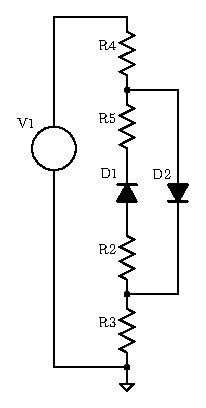
\includegraphics{c5}
\caption{Modified circuit.}
\label{fig:ex5}
\end{figure}

The result can be checked by exploring a modified circuit in which $R1$ and $R6$ have been removed.
Removing $R1$ and $R6$ effectively sets their value to infinity in which case the statement (\ref{eq:db2}) will most certainly be true. 
Figure \ref{fig:ex5} shows the circuit with $R1$ and $R6$ removed.
It is clear by inspection that diode $D1$ will be forward biased and diode $D2$ will be reverse biased when $V_{V1}$ is negative.

\section{A summary of the method}
The method that we used to extract information from the sparse matrix circuit model when it contains one or more ideal diodes can be summarized as follows:
\begin{enumerate}
\item Build the augmented sparse matrix including selector entries for the diodes.
\item Construct a solutions table with a row for each of the selector cases. 
Add columns for all of the diode voltages and currents. 
Add a column for each of any other desired solution variable.
\item Calculate the symbolic determinant of the sparse matrix.
\item Evaluate the determinant for each row. 
Remove any rows in which the determinant is identically zero. 
Append constraints to rows as required to insure that the determinant is never zero.
\item Solve the augmented sparse matrix symbolically .
\item Evaluate each solution variable in each row of the solutions table.
\item Update the constraints in each row as required by the diode characteristic implications.
\item Restate the constraints in terms that do not include any of the solution variables.
\item Combine each row of the solutions table in a final solutions statement that removes any overlapping cases.
\end{enumerate}

\section{Conclusion} 
We have presented a mixed data-type characterization for the (non-linear) ideal diode.
This characterization can be used with a generalized sparse matrix circuit model and symbolic mixed data-type solutions can be extracted from the resulting model.
Using the circuit model and the process of extracting solutions proceeds mechanically, using only the rules of mathematics and mathematical logic.

\section*{Acknowledgment}
This work was supported by XXXXXXX.

\bibliography{circuit}

\vspace{20pt}
\flushleft
\copyright 2004 XXXXX\\
email: XXXXXX\\

\end{document}
